\documentclass{ieeeaccess}
\usepackage{cite}
\usepackage{amsmath,amssymb,amsfonts}
\usepackage{algorithmic}
\usepackage{graphicx}
\graphicspath{{Images/}}
\usepackage{textcomp}

\usepackage[english]{babel}
\usepackage[utf8]{inputenc}
\usepackage[T1]{fontenc}
\usepackage{csquotes}
\usepackage{float}
\usepackage{enumerate}
\usepackage{lmodern}

\setlength{\marginparwidth}{2cm}
% \usepackage[disable]{todonotes}
\usepackage[showframe=false]{geometry}
\usepackage{amsthm}
\usepackage{subfiles}

\usepackage{siunitx}
\usepackage{multirow}
\usepackage{lscape}
\usepackage{booktabs}
\usepackage{tabularx} 
\usepackage[nottoc,numbib]{tocbibind}
\usepackage[super]{nth}

\usepackage[colorlinks=true, allcolors=blue]{hyperref}
\usepackage{xurl}

\usepackage{authblk}
\usepackage{changepage}

\usepackage[labelsep=period]{caption}
\usepackage[justification=centering]{caption}
\usepackage{soul}

% \captionsetup[table]{name=TABLE}
\renewcommand{\thetable}{\Roman{table}}

\hyphenation{Block-cha-in}
\hyphenation{block-cha-in}

\newtheorem*{rqa1}{RQA1}
\newtheorem*{rqa2}{RQA2}

\newtheorem*{rqb1}{RQB1}
\newtheorem*{rqb2}{RQB2}

\newtheorem*{rqc1}{RQC1}
\newtheorem*{rqc2}{RQC2}
\newtheorem*{rqc3}{RQC3}
\newtheorem*{rqc4}{RQC4}

\setlength\extrarowheight{2pt}

\def\BibTeX{{\rm B\kern-.05em{\sc i\kern-.025em b}\kern-.08em
    T\kern-.1667em\lower.7ex\hbox{E}\kern-.125emX}}
\begin{document}
% \history{Date of publication xxxx 00, 0000, date of current version xxxx 00, 0000.}
\doi{10.1109/ACCESS.2023.0322000}

\title{Impact of Decentralisation on Electronic Voting Systems: A Systematic Literature Survey}
\author{\uppercase{Ricardo Lopes Almeida}\authorrefmark{1,2}, 
% \IEEEmembership{Fellow, IEEE},
Fabrizio Baiardi\authorrefmark{2},
Damiano Di Francesco Maesa\authorrefmark{2} \IEEEmembership{Fellow, IEEE}, 
% \IEEEmembership{Member, IEEE}
Laura Ricci\authorrefmark{2}
}

\address[1]{Universit\'a di Camerino, 62032 MC, Camerino, Italy (e-mail: ricardo.almeida@unicam.it)}
\address[2]{Dipartimento di Informatica, Universit\'a di Pisa, 56127 PI, Pisa, Italy}

% \tfootnote{This work was supported in part by the U.S. Department of Commerce under Grant BS123456.}

% \markboth
% {Author \headeretal: Preparation of Papers for IEEE TRANSACTIONS and JOURNALS}
% {Author \headeretal: Preparation of Papers for IEEE TRANSACTIONS and JOURNALS}

\corresp{Corresponding author: Ricardo Lopes Almeida (e-mail: ricardo.almeida@unicam.it).}


\begin{abstract}
    The modernization of voting methods is a dynamic area of research currently. In the past, innovation in voting methods was limited to the automation of steps in the process through mechanical means. This changed with the introduction of commercial cryptography in the 1970s, whose applications to voting triggered a new era in this research field. Researchers used the following years to apply tools derived from cryptographic methods to build increasingly secure, transparent, and practical electronic voting systems. Despite the effort, a true remote electronic voting system was never achieved with the technology available. The introduction of Bitcoin in 2009 brought much attention to the blockchain concept that supported it. This new data model offered new levels of transparency, data immutability, and pseudo-anonymity that made it attractive and useful to e-voting researchers. Soon after, articles detailing the first blockchain-based e-voting systems were published, and the research field entered a new era. This article presents a study on the evolution of research in electronic voting systems, following a systematic literature review methodology and a chronological evolution from the first systems that employed public cryptographic concepts up to blockchain-based proposals, with the objective of detailing the evolution of the technology as a whole, as well as all the elements, centralised and decentralised, created and used to implement voting systems.
\end{abstract}

\begin{keywords}
blockchain, cryptography, e-voting, survey, systematic literature review
\end{keywords}

\titlepgskip=-21pt

\maketitle

\section{Introduction}
    \label{sec:introduction}
    Modern democracies provided societies with levels of comfort and security that enabled their citizens to move on from simply surviving to engaging in high-level intellectual activities. This fostered scientific and technological advancements that systematically upgraded almost all societal aspects. Amid such innovations, voting as an exercise remains largely unaltered, even in advanced democracies. Voting exercises may have evolved from dropping pebbles into clay pots \cite{Jones2003} to touching a virtual button on a touchscreen, but the essence of the process has not changed significantly. The nature of this exercise makes it a hard one to upgrade.
    \par
    Regardless of the lack of innovation in the voting process itself, voting systems have been the object of academic research. Developments in computer-based cryptography opened new research avenues, with electronic voting systems being one of the beneficiaries. The mechanisation and automation of voting systems is an old topic, but advancements in this field were restricted to supporting existing voting systems. Therefore, in essence, not much changed from the voter's perspective.
    \par
    Until recently, research on this topic followed a centralised design paradigm under a "classic" server-client architecture. These systems used cryptographic methods to blind sensitive information within the system, with the bulk of the computations reliant on a central computational unit, or cluster. So far, researchers have been unsuccessful in conceiving a secure, transparent, and scalable e-voting system that also addresses voter mobility and could translate into a widely adopted real-world application. This problem increases in importance when one considers modern levels of human mobility and emigration.
    \par
    An initial surge of cryptography-based voting systems was followed by a steady stream of improvements over older proposals, mostly due to technological advancements in subsequent years. This tendency remained unchanged until 2009, when the world's first cryptocurrency, Bitcoin, and the decentralised design paradigm brought along by blockchain technology \cite{Nakamoto2008} that supported it were introduced. In simple terms, a blockchain is a data structure replicated and distributively managed across a number of active machines, or nodes, in a computer network. Data is written into discrete blocks that are cryptographically chained linearly together, hence the name. Blockchain protocols employ the same cryptographic techniques used by centralised e-voting systems to achieve voter privacy, system transparency, universal verifiability, etc. in their basic mechanics. Therefore, it is possible to tap into these native features to implement transparency and data immutability in a voting system, something that requires dedicated resources in a centralised model. Blockchain did not need to wait too long to make its impact within e-voting research, with the first blockchain-based e-voting proposal appearing less than a decade after Bitcoin's debut. The analysis executed in Section \ref{3_slr_decentralized} explores these early proposals and how they evolved into more mature and realistic solutions over this period.
    \par
    This work intends to provide a systematic analysis of the evolution of the e-voting research field, with particular emphasis on how the introduction of the decentralised design paradigm influenced academic research on this topic. To achieve this goal, we have split the publications considered into centralised and decentralised proposals, the latter denoting blockchain-based solutions solely. The analysis of these works is framed under a \textit{systematic literature review (SLR)} \cite{Kitechenham2009} \cite{Petersen2008} \cite{Tranfield2003} approach, with a detailed classification, selection, and characterisation criteria detailed in the following sections, framed around a set of research questions, followed by the analysis to answer them.
    \par
    This article follows the structure outlined in Fig. \ref{fig:paper_structure}:


    \begin{figure}[h!]
        \centering
        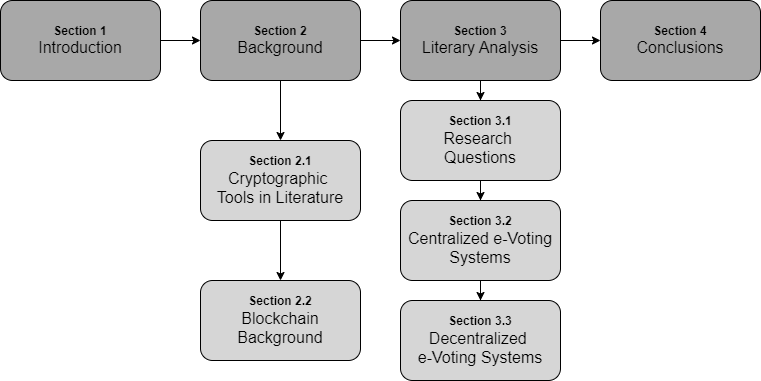
\includegraphics[width=\columnwidth]{Images/almei1.png}
        \caption{Survey article structure.}
        \label{fig:paper_structure}
    \end{figure}

    \section{Related Works}
    \label{related_works}
    Literature surveys on e-voting systems before the introduction of blockchain protocols are few. \cite{Bungale2003} is the oldest publication on the topic we could find. It is a brief report exploring the problem by considering the state of academic research and presenting practical cases where some form of electronic voting has been used in a real-world scenario. In 2003, most of these examples were limited to the use of DRE (direct recording electronic) voting machines. \cite{Weldemariam2010} presents the first academic survey of this kind, but this publication is centred on the technological details of DRE voting machines more than the theoretical academic approaches to the problem. This approach was emulated in \cite{OMeara2013}, which presents a more exhaustive approach to DRE voting machine applicability as well as an analysis of the outcome of real-world elections where these devices were used. An interesting addition to this publication is the formalisation of a series of "desirable e-voting system properties", which are then used to frame the analysis of real-world implementations. \cite{AlSammak2015} follows a similar strategy, defining a set of "requirements of e-voting", which follow closely on the set considered in \cite{OMeara2013}. But, as the title implies, the authors are mostly focused on the societal and technological challenges foreseen in the implementation of such systems. Regarding the formalisation of criteria used to classify e-voting systems, \cite{Ali2016} presents the most complete analysis to date in this regard. The authors used the additional space provided by publishing their research in a book chapter to present a detailed list of classification criteria, named "Security Properties of Voting Systems", which are quite similar to the set determined in Section \ref{minimum-classification-criteria}.
    \par
    Contrary to the pre-blockchain era, literature surveys on blockchain-based e-voting systems are more popular. The first publication that we found that could fit this mould was \cite{Nasser2018}. Published in 2018, this white paper does a somewhat comprehensive survey on existing e-voting technology, of which the vast majority still fell under the centralised approach. The authors proceed to explore how adding a blockchain to these earlier proposals may solve some of the identified problems, but they make no attempt to review any of the early blockchain-based proposals that were already published. This article was followed shortly by more thorough surveys: \cite{Kadam2019} and \cite{Sayyad2019} presented short surveys, while \cite{Abuidris2019} continues the trend of defining classification criteria to characterise e-voting systems, now under a decentralised, blockchain-based approach. However, the publication set considered in that work is too small to determine any valuable trends. This publication also provides a short overview of the real-world applications of blockchain-based e-voting systems, an element overlooked in most surveys.
    \par
    In \cite{Tas2020}, we found a good example of a systematic literature review covering a subset of the same publications considered in this work. The authors do formalise a set of classification criteria, following the same logic as previous authors, but their analysis focuses only on the cryptographic characteristics of blockchain-based e-voting systems and other practical elements, not on the implementation of these criteria by the solutions reviewed.
    \par
    The adoption of classification criteria for e-voting systems does become more apparent in later blockchain-based surveys. Publications such as \cite{Rabia2021}, \cite{Vivek2020}, \cite{Cabuk2020}, and \cite{Jafar2021} provide good examples of this strategy, which produce quite similar works, often diverging mostly on the publication set considered for analysis.
    
    \subsection{Research Gaps}
    \label{research-gaps}
    Blockchain-based e-voting systems have been properly surveyed during their short window of existence, but the same cannot be said for their pre-blockchain counterparts. As we have indicated in Section \ref{related_works}, the few surveys found under this classification are mostly focused on practical applications of e-voting technology through its application in DRE voting machines, or they consider publication sets much smaller and/or limited to a single computational approach.
    \par
    Another gap that we identified was the lack of a formal definition of the basic properties that an e-voting system should have, regardless of the actual implementation. \cite{Ali2016} provides a complete analysis in this regard, but it is limited to centralised proposals. No other survey extends this analysis to both paradigms. In other surveys, the criteria set considered is still too informal and subjective to be used as a standard classification method for these works. The type and nature of the criteria used to characterise an e-voting system are highly variable from author to author, both in concrete proposals and in surveys. Though most authors tend to elaborate their list based on past references, they do take liberties to change the criteria at will, which complicates any effort to find a consensus.
    \par
    Finally, a need for a chronological analysis was also identified related to the evolution of these systems, considering the overlap in terms of cryptographic techniques implemented. We consider an analysis from this point of view important, as it allows us to infer future trends for this technology.
    
    \subsection{Our Contribution}
    The contributions of this work are directly related to the research gaps identified. As far as we could discern, this is the first survey that covers the complete history of e-voting system development. The articles that we considered for our analysis include the earliest publications that used commercial cryptography to establish secure voting channels, up to the latest proposals based on smart-contract-enabled blockchain protocols. Along with such extensive analysis, we used a significantly larger publication set to discern chronological trends that become apparent with a systematic approach.
    \par
    Our work also provides a systematisation of the set of criteria used by the selected authors to characterise their solutions. As it was indicated previously in Section \ref{research-gaps}, there is a clear lack of standardisation around these criteria. During the systematic literature review, we grouped the criteria used by authors into a smaller set of broader criteria with the objective of establishing a more clear picture of the proper classification of these systems.
    \par
    We applied a uniform characterization framework derived from the uniformization effort around the classification criteria to all publications considered. We also presented an innovative analysis that characterises the e-voting systems considered using a standardised classification method and applied the same logic to e-voting proposals from both computational approaches considered. In addition, our analysis of blockchain-based e-voting systems provides a characterization in much greater detail than previous works of this type. In this regard, we considered a much larger publication set when compared with similar works and an extended characterization set for a decentralised approach that provides a more detailed account of the evolution of research in this field. As far as we could determine, ours is the first survey of this kind to present a literary analysis with such an extended publication set, as well as framing this analysis under a research period defined by two types of computational approaches.

\section{Background}
    \label{background}
    Prior to moving into the main literature analysis, we detail the cryptographic tools identified across the literature considered. These tools are transversal to both the considered paradigms and are critical for the understanding of our analysis, especially for readers that are not familiar with general cryptography.
    \par
    The focus of this paper is to characterise and organise how proposals for e-voting systems use cryptographic tools to ensure the security of their usage of the systems proposed. Though there are abundant non-cryptographic methods to achieve this goal, our analysis is centred only on the ones that are based on cryptographic primitives.
    
    \subfile{./Sections/1_Background.tex}
    \label{cryptographic_methods}

    \section{Literature Analysis}
\label{literature-analysis}
Following the \textit{Systematic Literature Review (SLR)} guidelines established in \cite{Kitechenham2009}, \cite{Petersen2008}, and \cite{Tranfield2003}, literature in both the centralised and decentralised domains was analysed in order to extract common characteristics and technological trends.
\par
This literature analysis was split into two sections:
\begin{enumerate}[I]
    \item \textbf{Centralised e-voting systems} For publications detailing architectures that fall under the traditional server-client model.
    \item \textbf{Decentralised e-voting systems} For more recent publications that used blockchain implementations to base their systems on, thus following a decentralised design approach.
\end{enumerate}

\subsection{Research Questions}
\label{research-questions}
\subsubsection{General Research Questions}
\label{general-research-questions}
To set boundaries for this review, we established sets of research questions to be answered with the analysis of each paradigm. Due to the fact that the decentralised design evolves from the previous, centralised one, we begin by establishing a set of broader research questions that can be applied to both approaches:
\par
\vspace{0.25cm}
\textbf{On Security Criteria Implemented:}
    \begin{rqa1}
        What are the security criteria for electronic voting systems that are consistently addressed in the research literature?
    \end{rqa1}

    \begin{rqa2}
        Which security criteria are implemented at higher rates in the proposals considered?
    \end{rqa2}

\textbf{On Cryptographic Methods Identified:}
    \begin{rqb1}
        What are the main cryptographic tools used by the e-voting systems analysed?
    \end{rqb1}

    \begin{rqb2}
        Which cryptographic tools identified in academic proposals were used in real-world e-voting implementations?
    \end{rqb2}

\subsubsection{Decentralized Proposals-specific Research Questions}
\label{specific-research-questions}
Proposals under the decentralised paradigm are also going to be analysed based on the security criteria, albeit with an adapted set, and the usage of cryptographic methods is also adapted to the new paradigm. The differences between them justify adding a new set of research questions to establish clear boundaries for the analysis of the latter:
\par
\vspace{0.25cm}
\textbf{On Decentralised Proposal Characteristics:}
    \begin{rqc1}
        Which blockchain type and access control are used in decentralised e-voting solutions?
    \end{rqc1}

    \begin{rqc2}
        Are smart contracts used in the decentralised e-voting proposal?
    \end{rqc2}

    \begin{rqc3}
        Are there any centralising elements in the proposed solution?
    \end{rqc3}

    \begin{rqc4}
        What are the methods used in blockchain-based e-voting systems to cast votes?
    \end{rqc4}

Each section begins by establishing a frame of analysis based on the applicable set of \textit{research questions} defined so far, establishes the criteria necessary to answer these, performs the literature analysis, and concludes with a survey of real-world system implementations and respective analysis.

    \subsection{Centralised e-Voting Systems}
        \label{centralized_solutions}
        \subfile{./Sections/2_SLR_Centralized.tex}

    \subsection{Decentralised e-Voting Systems}
        \label{decentralized_solutions}
        \subfile{./Sections/3_SLR_Decentralized.tex}

\twocolumn

\section{Conclusions}
This study illustrates how research into modernising voting systems divides into two overlapping eras, with each one triggered by a landmark article that introduced technological principles that allowed new research. Diffie and Hellman's \cite{Diffie1976} 1976 publication brought computer cryptography to the public realm and with it a steady stream of innovations, not just towards more secure e-voting systems but also benefiting a plethora of industries and applications. And the same seems to be happening again with Satoshi Nakamoto's \cite{Nakamoto2008} 2009 publication. The paradigms explored are neither exclusive nor denote a sudden shift from one to the other. Instead, they reflect how e-voting research has evolved through the years, as it is able to successfully incorporate new technological advances to further its own.
\par
Decentralised proposals benefited greatly from the previous, centralised ideas in the sense that these have cleared plenty of cryptographic hurdles that paved the way for the current landscape of decentralised e-voting research. Ideas that were somewhat foreign and unfamiliar decades before, such as encryption methods, homomorphism, and one-way hash functions, are now commonplace within the new era of e-voting solutions, in great part due to the efforts of early researchers.
\par
We have observed a closer relationship between academic proposals and real-world implementations with the decentralised paradigm than with its centralised counterpart, which is an objectively positive trend. Yet, both paradigms are still unable to provide an e-voting solution that could really complement existing voting methods and, perhaps, even replace them in the future. None of the systems indicated in Section \ref{real-world-centralized} is in use today, despite their relative success. All the information obtained thus far relating to the examples indicated in this section points to a discontinuation of the trials, and the lack of more recent examples of centralised e-voting systems being used, either as an official voting method or on an experimental basis, reinforces this notion.
\par
The decentralised solutions indicated in Section \ref{real-world-decentralized-solutions} have a closer relationship to their academic counterparts, but most of them were found to have never been used, or even ready for, a large-scale election setting. The sole exception is Agora, which claims to have taken part in Sierra Leone's 2018 presidential elections. But a statement issued by the company \cite{Agora2018} indicates that the involvement of this company was minimal, namely, that it acted mostly in the capacity of an international observer and that the deployment of their technology in those elections was partial, at best. The main objective of this exercise was to demonstrate the system's capabilities in order to achieve further cooperation opportunities with Sierra Leone's National Election Commission. The remaining solutions considered are still untested in a real-world scenario at the time of this writing.
\par
Though the paradigms are getting increasingly successful in tackling problems of trust that may prevent wide adoption of a truly remote e-voting system, it appears that the efforts undertaken so far are still insufficient. But the technological landscape that we described in this document is still changing. Technological advances such as highly scalable and efficient public blockchains and the Non-Fungible Token Standard are creating promising research avenues.
This is particularly relevant for the decentralised approach, where we could identify a chronological progression with the solutions analysed. Early solutions try to adapt a financial tool for alternative purposes, which shows in their lack of applicability. As the technology evolved and researchers had more tools to use, solutions became more elegant and more fitted to the purpose, rather than being limited to adjusting something that was being used for another purpose to a different application. Smart contract usage is a good example of this tendency. Their applicability to e-voting solutions is such that they became almost ubiquitous soon after being introduced.

\bibliographystyle{IEEEtran}
\bibliography{surveyBibliography}

\begin{IEEEbiography}[{
\includegraphics[width=1in,height=1.25in,clip,keepaspectratio]{almei1.png}}]{Ricardo Lopes Almeida} is a doctoral student in the first edition of the Italian Doctoral Programme in Blockchain and Distributed Ledger Technology - Social Systems and Smart Societies at the Univesità di Pisa and Università di Camerino. He obtained an Integrated Master's in Electronic Engineering and Telecommunications from the University of Aveiro, Portugal, in 2012 and a graduation in Physics and Chemistry from the University of \'Evora, Portugal, in 2005.
\par
He has split his career almost evenly between academia and industry. He has worked as a science teacher in public schools and as a private tutor. After acquiring a qualification as an engineer, he has worked mainly as a consulting software developer and telecommunications engineer. 
\end{IEEEbiography}

\begin{IEEEbiography}[{\includegraphics[width=1in,height=1.25in,clip,keepaspectratio]{baiar1.png}}]{Fabrizio Baiardi} graduated in computer science at Universit\'a di Pisa where he is currently a full professor in computer science.
\par
His main research interest is cyber risk assessment and management. He is a cofounder of Haruspex, a startup that develops risk assessment and management tools based upon adversary emulation. He holds some patents on intrusion detection.
\end{IEEEbiography}

\begin{IEEEbiography}[{
\includegraphics[width=1in,height=1.25in,clip,keepaspectratio]{maesa1.png}}]{Damiano Di Francesco Maesa} is an assistant professor in computer science at the University of Pisa, Italy. His past affiliations include the University of Cambridge, King's College London, and the National Research Institute of Italy.
\par
He has a PhD in Computer Science from the University of Pisa and specialises in blockchain and Distributed Ledger Technologies (DLT). He has been involved in the topic since 2013, and, beside his academic contributions, he has held several guest lectures, seminars, and workshops to spread awareness about blockchain technology.
\end{IEEEbiography}

\begin{IEEEbiography}[{
\includegraphics[width=1in,height=1.25in,clip,keepaspectratio]{ricci1.png}}]{Laura Ricci} received the M.Sc. in Computer Science from the University of Pisa in 1983 and the Ph.D. from the same university, in 1990. She is currently a full professor at the Department of Computer Science, University of Pisa, Italy.
\par
Her research interests include cryptocurrencies and blockchains, peer-to-peer networks, and social network analysis. In these fields, she has co-authored 150+ papers published in international journals and conference/workshop proceedings. She has served as programme committee member and chair of several conferences and workshops. She has been involved in several research projects, and she is currently the coordinator of the Italian PRIN project "AWESOME: Analysis framework for WEb3 SOcial MEdia". She has been a member of the National Committee for the definition of the Italian National Strategy for Blockchain.
\end{IEEEbiography}

\EOD
\end{document}
